% =====================================================================
% NeurIPS workshop submission.
% Drop the workshop's official style file (e.g. neurips_2026.sty) next to
% this file. Compiles with pdflatex + bibtex.
% All families are evaluated OUT-OF-SAMPLE on the same shared held-out
% trajectories (movement_id); references.bib verified against arXiv (June 2026).
% =====================================================================
\documentclass{article}

% Double-blind submission to the NeurIPS 2026 TAE (Trust-AI-Eval) workshop.
\IfFileExists{neurips_2026.sty}{%
  \usepackage[dblblindworkshop]{neurips_2026}%
}{%
  \usepackage[margin=1in]{geometry}\usepackage{parskip}\usepackage{natbib}%
  \providecommand{\workshoptitle}[1]{}%
}

\usepackage[utf8]{inputenc}
\usepackage[T1]{fontenc}
\usepackage{hyperref}
\usepackage{url}
\usepackage{booktabs}
\usepackage{amsfonts,amsmath,amssymb}
\usepackage{microtype}
\usepackage{graphicx}
\usepackage{pgfplots}
\pgfplotsset{compat=1.18}
\usepackage{xcolor}
\usepackage{siunitx}
\usepackage{multirow}
\usepackage{enumitem}

\title{Correct Scores, Wrong Conclusions:\\
Auditing Forecasting Benchmarks on Chaotic Dynamics}
\workshoptitle{TAE (Trust-AI-Eval): Can We Trust AI Evaluation?}

% Anonymized for double-blind review. At camera-ready, restore the TWO-author
% list below. Do not reinstate the earlier three-author list: Shrithik Shahapure
% is a non-author contributor (compute access for the Azure AI Foundry LLM
% evaluations and help running them), credited in Author Contributions.
%
% \author{%
%   Sriman Narayan Kandi\thanks{Corresponding author.}\\
%   Independent Researcher
%   \And
%   Trishant Srinivasan\\
%   Independent Researcher
% }
\author{}

\begin{document}
\maketitle

\begin{abstract}
Forecast accuracy does not by itself establish scientific forecasting ability. We test five
conditions that connect a score to a scientific claim: held-out generalization, complete
failure accounting, matched disclosure, structural identifiability, and cross-system
transfer. We apply these tests to $k$-pendulum ($k\in\{1,2,3\}$) and Lorenz--63 forecasts from
language models, a time-series foundation model, learned dynamics, sparse identification, and
numerical integrators. Each test changes a substantive conclusion. Learned-model error rises
from $0.09$--$0.63$\,rad on training trajectories to $0.97$--$1.14$\,rad on held-out
trajectories, where linearized dynamics and nearest-neighbor lookup perform better. Retaining
failed forecasts lowers the reported performance of models with incomplete coverage. An
unmatched comparison says that hiding physical constants helps; a paired intervention instead
finds a small, model-dependent effect (pooled $+0.069$\,rad; $+0.211$ to $-0.042$ across models). Two exact scale symmetries prove that the absolute constants are
not identifiable from angle trajectories. Increasing the Neural~ODE training set improves
error from $1.090$ to $0.861$\,rad but does not reach known-equation integration. The pendulum
ordering also fails to transfer to Lorenz--63, where SINDy recovers the polynomial dynamics to
numerical precision. On video-tracked hardware the roles invert: the RK4 model with published
constants is itself imperfect, and its lead over simple baselines is gone within a second.
These results show that a correct leaderboard can still support incorrect
scientific conclusions: an unaudited score does not earn trust. We release the prompts,
outputs, checkpoints, seeds, and compute records needed to repeat the audit.
\end{abstract}

\section{Introduction}
Scientific claims require more than low forecast error. A leaderboard states what was
measured, not what inference it supports: a result may depend on training trajectories,
dropped failures, unmatched inputs, an unidentifiable target, or one favorable system. We
study the evaluation protocol itself, not only the models it ranks. Given state $\mathbf{s}_t$, the task is to
predict $\mathbf{s}_{t+T}$. The $k$-link pendulum is integrable at $k{=}1$ and chaotic for
$k{\ge}2$, has high-precision ground truth, and permits controlled changes to physical
metadata. Lorenz--63 provides a second system with a different observation model and
hypothesis class; a hardware replication of the audit (\S\ref{sec:realdata}) scores the
reference model itself as the imperfect one.

Our contribution is a claim audit for dynamical-system forecasts. It scores only held-out
trajectories, counts every failed forecast, toggles disclosure on identical trajectories,
checks identifiability before scoring parameter recovery, and tests whether conclusions transfer
to a second system; throughout, it records the information each method receives, without which
none of the five is interpretable. The five are indexed to the claims, not drawn from a
taxonomy: each tests one inference step between a score and a conclusion (sample to population,
answered cells to full task, correlation to attribution, accuracy to parameter recovery, one
system to a family claim), and claims we do not make would need other checks, such as
calibration for probabilistic forecasts.
Table~\ref{tab:audit-summary} states the conclusion before and after each test. Empirically,
all five tests alter or reject a conclusion supported by the unaudited comparison, and at least
two of them concern conclusions drawn in practice: zero-shot forecasters are routinely scored
without failure accounting or matched controls
\citep{gruver2023llmtime,zhang2025zeroshotchaos}.

\begin{table}[tbp]
\centering\footnotesize\renewcommand{\arraystretch}{0.78}
\caption{Conclusions before and after the claim audit. Each row changes one part of the
evaluation while preserving the relevant model outputs or comparison set.}
\label{tab:audit-summary}
\begin{tabular}{p{0.16\linewidth}p{0.35\linewidth}p{0.39\linewidth}}
\toprule
Test & Unaudited conclusion & Audited conclusion \\
\midrule
Failures &
Answered forecasts represent model performance. &
Incomplete coverage lowers reliability-adjusted performance. \\
Generalization &
Learned dynamics forecast accurately. &
At this budget, held-out error is up to $11\times$ in-sample, and simple baselines perform better. \\
Disclosure &
Withholding constants improves forecasts. &
Matched, the effect is small and model-dependent ($+0.069$\,rad pooled). \\
Identifiability &
Absolute constants can be recovered from angles. &
Two exact symmetries make absolute recovery impossible. \\
Transfer &
The pendulum order ranks model families. &
Lorenz--63 produces a different order. \\
\bottomrule
\end{tabular}
\end{table}

\section{Related work}
\paragraph{Learned dynamics and foundation forecasters.} Neural~ODEs learn a continuous-time
vector field~\citep{chen2018node}; Hamiltonian and Lagrangian Neural Networks add
energy-conserving and Euler--Lagrange inductive biases~\citep{greydanus2019hnn,cranmer2020lnn};
chaotic systems are standard testbeds~\citep{gilpin2021chaos}. LLMs act as zero-shot forecasters
when series are serialized as text~\citep{gruver2023llmtime}, time-series foundation models such
as Chronos, TimesFM, and Moirai are trained for general forecasting~\citep{ansari2024chronos,das2024timesfm,woo2024moirai},
and \citet{zhang2025zeroshotchaos} apply them to chaotic systems. LLMs also do well on
mathematical~\citep{lewkowycz2022minerva,wei2022cot} and physics~\citep{xu2025ugphysics}
reasoning. We evaluate all of these on one grid.

\paragraph{Evaluation validity.} Our five checks are the standard validity questions of
measurement---internal (do failure accounting and matched controls isolate the effect), construct
(does the score measure forecasting rather than input access or an unidentifiable target), and
external (does a conclusion transfer). SINDy~\citep{brunton2016sindy} and
NVAR~\citep{gauthier2021nvar} supply an identification baseline; structural identifiability asks
which parameters are recoverable from observed outputs, including under
symmetries~\citep{borgqvist2024symmetries}; and unlike selective prediction, which reports risk
with coverage~\citep{geifman2017selective}, we keep failed cells in the score at fixed coverage.

\section{Benchmark design}
\paragraph{Choice of systems.} We use the $k$-link pendulum to vary the number of coupled links
while retaining a high-precision numerical solution. Its constants can also be hidden without
changing the underlying trajectory, which permits the matched test in \S\ref{sec:sysid}.
The smaller Lorenz--63 experiment repeats the local-model comparison on a second
chaotic system; the LLM and disclosure experiments were not rerun there.

\subsection{Task and systems}
Given the state $\mathbf{s}_0=(\theta_1,\dots,\theta_k,\omega_1,\dots,\omega_k)\in
\mathbb{R}^{2k}$ of a $k$-link pendulum at $t{=}0$, the task is to predict $\mathbf{s}_T$ at
horizon $T$. Ground-truth trajectories integrate the full nonlinear Lagrangian equations of
motion with fixed-step RK4 at $\Delta t{=}10^{-3}$\,s, recording states every $0.01$\,s plus
a $10$\,s pre-$t{=}0$ context window (used only by the time-series models). Initial
conditions are sampled $\theta_i\sim\mathcal{U}(-3,3)$\,rad,
$\omega_i\sim\mathcal{U}(-1,1)$\,rad/s with a fixed seed. Because the labels are produced by
RK4 at this step, the RK4 baseline reported later (the same integrator at a $10{\times}$
coarser $\Delta t{=}10^{-2}$) is a numerical reference by construction, not an independent
competitor. Euler and the symplectic integrator are distinct known-physics methods. Inputs
available to each family are stated in \S\ref{sec:inputs}.

\subsection{Regimes and grid}
Three regimes test generalization to non-standard constants (Table~\ref{tab:regimes}). In
\texttt{changed\_hidden} the constants $(g,L,m,d)$, with damping $d$, are not disclosed to the
model. This regime contrast is not matched---\texttt{changed\_hidden} differs in its constants
as well as in disclosure, so its trajectories differ in difficulty---which is why \S\ref{sec:sysid}
adds a disclosure toggle on identical trajectories. Withholding is nonetheless informative,
since a single state contains no observed dynamics from which to identify the constants. An evaluation cell is a tuple (model, $k$, regime,
horizon), with horizons $\{0.01,1,10,60\}$\,s. The full LLM grid also varies input modality
and prompting; every comparison here uses the coordinate modality with direct prompting
(the other axes are analyzed in Appendix~\ref{app:axes}).

\paragraph{Out-of-sample protocol.} Learned dynamics models are never scored on their training
data. We generate a shared held-out set (a separate seed from the training trajectories) of
$180$ initial conditions ($60$ per regime, spanning $k\in\{1,2,3\}$) and evaluate every
family on the identical trajectories, keyed by \texttt{movement\_id}. The cross-family
comparison (\S\ref{sec:reliability}) uses horizons $\{1,10\}$\,s, where chaos has begun but
error has not saturated (\S\ref{sec:metrics}), giving $180\times2=360$ cells per model;
in-sample error appears only once, to quantify the size of the generalization gap
(\S\ref{sec:reliability}).

\subsection{Inputs and grouping}
\label{sec:inputs}
Table~\ref{tab:inputs} states what each family receives. Chronos is a time-series model, so
we evaluate it in its standard form: a history-conditioned forecaster with a $10$\,s
pre-$t{=}0$ context window. The LLMs and learned dynamics models are state-conditioned from
$t{=}0$. For learned models, hidden-regime cells are equalized by withholding hidden constants
and using normal-regime prior constants. A separate asymmetry runs in the opposite direction:
the LLMs are large hosted models, whereas the learned models are small
($256$-wide, $3$-layer MLPs trained on a single $8$\,GB GPU; Appendix~B). The behavior of
larger physics-informed networks is outside this study's scope. We separate known-physics
methods (RK4, Euler, symplectic) from black-box methods (LLMs, Chronos, learned
dynamics); the former are numerical references.

\begin{table}[tbp]
\centering\small
\caption{Inputs available to each family. State is at $t{=}0$; history is pre-$t{=}0$.
Chronos-2 is history-conditioned; learned \texttt{hidden} cells withhold hidden constants.}\label{tab:inputs}
\begin{tabular}{lcccc}
\toprule
Family & State & History & Constants & Equations \\
\midrule
Numerical (RK4/Euler/sympl.) & \checkmark & --- & \checkmark\ (all regimes) & \checkmark\ (exact) \\
Learned (NODE/HNN/LNN) & \checkmark & --- & \checkmark\ base; withheld$^\ast$ & --- (learned) \\
Time-series (Chronos-2) & --- & \checkmark\ ($10$\,s context) & --- & --- \\
LLMs (kimi/grok/deepseek) & \checkmark & --- & \checkmark\ except \texttt{changed\_hidden} & --- \\
\bottomrule
\end{tabular}
\end{table}

\subsection{Metrics}
\label{sec:metrics}
The primary metric is mean absolute angle error (rad), wrapped to $[-\pi,\pi]$ and
averaged over links and trajectories; energy drift is reported separately (\S\ref{sec:energy}).

\paragraph{Reliability-adjusted error.} A cell is answered only if the model returns a
parseable, finite prediction. Reporting error over answered cells alone would reward
abstention on hard cells. We therefore assign unanswered cells the random-guess baseline
$\pi/2$ (the expected wrapped-angle error of a uniform guess); under the strict upper bound
$\pi$ only the incomplete-coverage models move (\S\ref{sec:reliability}). Answering is part
of the score: the task is fixed-coverage forecasting, not selective prediction. Angles alone
are scored, since wrapping gives answers and failures one bounded scale that unbounded
velocities lack.

\paragraph{Verification record.} For each evaluation cell we retain the trajectory identifier,
model and deployment name, prompt, raw response, parser outcome, prediction, prompt and
completion token counts, and score. The released configuration fixes the data-generation
solver, held-out seed, horizons, prompts, timeout, and temperature. Two standards apply here.
Local methods are reproducible: their checkpoints and seeds regenerate the predictions exactly.
Hosted models are not, because a deployment can change or be withdrawn between evaluations, so
for them the record is what remains. We therefore release the per-cell responses rather than
summary scores alone, which keeps the reported API evaluation auditable after the deployments
it measured are gone.

\paragraph{Predictability horizon.} For chaotic systems, pointwise error past the Lyapunov
time saturates to a system-dependent constant for every model, so long-horizon error
rankings carry little information. We define the predictability horizon as the longest
horizon a model tracks contiguously below a threshold $\tau$, starting from $t{=}0$: we walk
horizons in increasing order and stop at the first that exceeds $\tau$. The contiguous rule
is used because, after divergence, a later horizon can fall below $\tau$ by angle-wrap
coincidence. We sweep $\tau$.

\paragraph{Disclosure gap.} We define
$\Delta_{\mathrm{disc}}=\mathrm{err}(\text{hidden})-\mathrm{err}(\text{disclosed})$.
Positive values indicate a penalty for withholding constants. Because regime contrasts
confound disclosure with trajectory difficulty, we also run a matched experiment
(\S\ref{sec:sysid}) that toggles disclosure on identical trajectories.

\section{Methods}
\label{sec:methods}
\paragraph{LLMs.} We evaluate \texttt{kimi-k2.6}, \texttt{grok-4-1-fast-reasoning}, and
\texttt{deepseek-v4-pro} through an OpenAI-compatible API (hosted deployments, June~2026),
with a structured prompt (system description, disclosed constants where applicable, initial
state) and a JSON answer schema (Appendix~A). Each cell uses one temperature-$0$ call with a
uniform token and timeout budget; no best-of-$N$ aggregation is used. The LLM evaluation (Parts~A and~B, $3{,}960$ cells) records prompt and completion
token counts and has an estimated nominal API cost of \$110.38 under the pricing assumptions
in the released analysis script.

\paragraph{Time-series foundation models.} We run Chronos-2 (model card \texttt{amazon/chronos-2};
the Chronos family is introduced by \citealp{ansari2024chronos}) locally
on a single GPU in its standard history-conditioned form: the $10$\,s pre-$t{=}0$ context
window of all $2k$ state channels, resampled to at most $512$ points, forecasts to the target
horizon (prediction length $\le 64$ steps). The comparison uses \texttt{chronos-2} in
univariate and multivariate modes; the latter forecasts all $2k$ channels jointly. The
paired mode comparison uses $20$ trajectories per $(k,\mathrm{regime})$ cell.

\paragraph{Learned dynamics.} Neural~ODE, HNN, and LNN share a $256$-wide, $3$-layer tanh
MLP and integrate at inference with \texttt{scipy}. We compare two objectives: derivative
matching (MSE on finite-difference $\dot{\mathbf{s}}$) and rollout loss (MSE on the state
after $w$ Euler steps, with gradients through the unroll). We also use mixed-window rollout,
which trains on several window lengths jointly (Neural~ODE: $w\in\{10,50\}$; HNN:
$w\in\{5,20\}$). The LNN's loss requires second-order automatic differentiation; the LNN trains at
full scale ($67$k samples, hidden 256) on a CUDA GPU.
The primary models are trained on nine trajectories, one for each $(k,\mathrm{regime})$ cell
(Appendix~B). A nested budget study trains fresh Neural~ODE and HNN checkpoints with
$\{1,5,20\}$ trajectories per eligible cell and seeds $\{101,102,103\}$. The Neural~ODE
uses all nine cells; because damping violates Hamiltonian conservation, the HNN budget study
uses only the three undamped normal-regime cells. Every checkpoint is evaluated on the same
two held-out seeds.

\paragraph{Integrators.} Euler, RK4, and St\"ormer--Verlet (symplectic) at $\Delta
t{=}0.01$\,s using the exact equations of motion; their error is from discretization alone.

\paragraph{Baselines.} Four reference baselines use the same grid: persistence
($\theta_T{=}\theta_0$), constant velocity ($\theta_T{=}\theta_0{+}\omega_0T$), a
small-angle linearized model, and a nearest-neighbor analog forecast from the matching
$(k,\mathrm{regime})$ training trajectory. The nearest-neighbor baseline uses the same data as the
learned models.

On both held-out seeds (equal-weighted; \S\ref{sec:replication}) we also fit SINDy
with a degree-two polynomial library and
STLSQ, and nonlinear vector autoregression (NVAR) with two delays, degree-two features, and
ridge regression. Divergent rollouts are retained as failures and receive the same $\pi/2$
penalty.

\paragraph{Lorenz replication.} A secondary Lorenz--63 test compares numerical references,
persistence, SINDy, NVAR, a Neural~ODE trained on $20$ single-seed trajectories, and zero-shot
Chronos-2 on five five-trajectory held-out seeds at $\{0.1,0.5,1.0\}$\,s (full configuration in
Appendix~C). The metric is coordinate MAE normalized by each Cartesian coordinate's training
standard deviation, averaged over coordinates and horizon (an error of $1$ is one training
standard deviation). HNN and LNN are omitted: Lorenz--63 is dissipative and non-Hamiltonian.

\section{Results}
\subsection{Failure accounting and held-out generalization}
\label{sec:reliability}
The shared held-out grid contains $360$ cells: 180 trajectories at horizons $\{1,10\}$\,s.
Every model is evaluated on that grid. The Answered column in Table~\ref{tab:overall} gives the
fraction of cells with valid predictions.
Confidence intervals are $95\%$ percentile bootstrap intervals from $B{=}10^4$ resamples of
whole held-out trajectories (both horizon cells together), paired across models on a common
resample; they are marginal per model, not simultaneous over the $19$ rows, and for LLMs
exclude per-call sampling variation.

Table~\ref{tab:overall} ranks the models on the pendulum under the access conditions in
\S\ref{sec:inputs}. The ranking is conditional on those inputs, this training budget, and this
system; Section~\ref{sec:lorenz} tests whether it transfers. The numerical integrators sit at the top as
references (RK4 $0.059$ at a finer step, symplectic $0.205$, Euler $0.405$),
and every learned-dynamics model lands closer to the $\pi/2$ random baseline than to the
RK4 and symplectic references. The lowest-error black-box entry is \texttt{kimi}
($0.538$\,rad, $98\%$ answered), whose interval is disjoint from the strongest baseline's
(nearest-neighbor, $0.725$).
That is a statement about one recorded June~2026 deployment under these evaluation
conditions, not about model families; the Lorenz test rejects the family reading.

Under the equalized hidden-regime run, nearest-neighbor lookup ($0.725$) beats every learned
model with a disjoint interval; the linearized pendulum ($0.855$) and persistence ($1.004$) sit
above every learned model but HNN-rollout ($0.972$) on point estimates, with marginal intervals
that overlap near the boundary. The stable learned models
score $0.09$--$0.63$\,rad on their training trajectories against $0.97$--$1.14$ held out
(Table~\ref{tab:insample}), a $1.7$--$11\times$ gap widest for the in-sample winner,
the mixed-window Neural~ODE.

Two further data-driven methods appear only on the two-seed replication subset, so we report them
in Table~\ref{tab:replication} rather than in the main comparison, and their scores must be read
with their coverage: SINDy answers $61\%$ of cells and scores $0.883$\,rad on that subset, and
NVAR answers $46\%$ and scores $1.248$. Because unanswered cells take the $\pi/2$ penalty, a
majority of NVAR's score and a substantial part of SINDy's is imputation rather than forecast
error, so these entries rank rollout stability together with accuracy.

\begin{table}[tbp]
\centering\footnotesize\renewcommand{\arraystretch}{0.74}
\caption{Out-of-sample cross-family comparison on the shared held-out set ($360$ cells, horizons
$\{1,10\}$\,s). Reliability-adjusted mean angle error (rad): unanswered or missing cells
scored at $\pi/2$; $95\%$ bootstrap CI. Inputs differ by family (Table~\ref{tab:inputs}); the
ranking is conditional on them, this budget, and this system. RK4 generates the data and is
included as a numerical reference. Configurations first evaluated in this work are marked $\dagger$;
simple baselines are marked $\ddagger$.}\label{tab:overall}
\begin{tabular}{rlcccl}
\toprule
\# & Model & Err & 95\% CI & Answered & Family \\
\midrule
-- & rk4 (reference) & 0.059 & [0.032, 0.089] & 100\% & numerical \\
1 & symplectic & 0.205 & [0.163, 0.251] & 100\% & numerical \\
2 & euler & 0.405 & [0.344, 0.470] & 100\% & numerical \\
3 & kimi-k2.6 & 0.538 & [0.475, 0.602] & 98\% & LLM \\
4 & chronos2-multi$^\dagger$ & 0.684 & [0.617, 0.752] & 100\% & time-series \\
5 & chronos2-uni$^\dagger$ & 0.697 & [0.631, 0.766] & 100\% & time-series \\
6 & nearest-neighbor$^\ddagger$ & 0.725 & [0.657, 0.797] & 100\% & baseline \\
7 & linearized$^\ddagger$ & 0.855 & [0.774, 0.939] & 100\% & baseline \\
8 & grok-4-1-fast-reasoning & 0.881 & [0.805, 0.957] & 82\% & LLM \\
9 & deepseek-v4-pro & 0.952 & [0.881, 1.027] & 100\% & LLM \\
10 & hnn-rollout & 0.972 & [0.898, 1.047] & 100\% & learned \\
11 & persistence$^\ddagger$ & 1.004 & [0.934, 1.078] & 100\% & baseline \\
12 & neural-ode-rollout-mixed$^\dagger$ & 1.036 & [0.967, 1.104] & 100\% & learned \\
13 & hnn-rollout-mixed$^\dagger$ & 1.066 & [0.990, 1.143] & 100\% & learned \\
14 & neural-ode & 1.110 & [1.039, 1.181] & 100\% & learned \\
15 & neural-ode-rollout & 1.121 & [1.054, 1.190] & 100\% & learned \\
16 & hnn & 1.138 & [1.059, 1.218] & 100\% & learned \\
17 & constant-velocity$^\ddagger$ & 1.319 & [1.241, 1.396] & 100\% & baseline \\
18 & lnn$^\dagger$ & 1.356 & [1.282, 1.430] & 94\% & learned \\
\bottomrule
\end{tabular}
\end{table}

\paragraph{Effect of missing predictions.} \texttt{grok} answers $82\%$ of the grid and
\texttt{lnn} $94\%$: their ranks fall when missing cells receive $\pi/2$. On answered cells
alone \texttt{grok} scores $0.729$ rather than $0.881$, ahead of every learned model; fixed
coverage keeps its abstentions in the score. Under the strict $\pi$ bound the LNN stays last
and \texttt{grok} falls eight places, while full-coverage models are unchanged. The order among
full-coverage models is invariant to the imputation constant; the rank of an incomplete-coverage
model is not, which is why coverage enters the score. A prompting change shows the same
mechanism: chain-of-thought leaves the ordering unchanged but is worse for the best LLM
($+0.121$\,rad, CI $[+0.061,+0.183]$) because its unanswered cells rise from $6$ to $50$,
moving the score through coverage, not accuracy (Appendix~\ref{app:axes}).

\subsection{Matched disclosure and identifiability}
\label{sec:sysid}
On the shared held-out set the hidden regime has lower error than the disclosed regime
($-0.390$\,rad, $p_{\mathrm{Holm}}{<}10^{-3}$, unpaired) and than the normal regime
($-0.524$). This looks favorable to withholding constants, but the regimes use different
trajectories, and the hidden ones are slower and less divergent, so the comparison cannot
speak to parameter recovery. When we instead toggle disclosure on identical trajectories for
the three LLMs ($900$ paired cells on a separate matched grid; Table~\ref{tab:sysid}), the
pooled sign changes: hiding the constants raises error by a small amount
($\Delta_{\mathrm{disc}}{=}{+}0.069$\,rad, $p_{\mathrm{Holm}}{=}0.034$, six tests). This pooled
figure averages heterogeneous per-model effects ($+0.211$, $+0.038$, $-0.042$) and is carried by
$k{=}1$ ($+0.297$; $k{=}2$ and $k{=}3$ reverse), so it bounds any penalty as small rather than
estimating one. The unadjusted hidden-regime advantage is therefore due to trajectory
difficulty, not disclosure.

The disclosure test also has a structural limit. The angular equations are unchanged by
$(m,d)\mapsto(am,ad)$ and by $(L,g,d)\mapsto(bL,bg,b^2d)$, so for $k{=}1$ only $g/L$ and
$d/(mL^2)$ are identifiable from an angle trajectory; absolute $g$, $L$, $m$, and $d$ cannot
be scored as independently recoverable. Asked to name the constants from a single state, the
LLMs mostly return Earth-standard defaults, which is evidence of a prior, not of recovery
(transcripts in the released records). A released check verifies both invariances to below
$10^{-13}$.

\subsection{Replication across seeds and training budgets}
\label{sec:replication}
We reran the local pendulum subset on an independent held-out seed with five trajectories per
$(k,\text{regime})$ cell; the original seed has 20. Table~\ref{tab:replication} reports each
seed separately and gives their unweighted mean. Three facts are seed-invariant: the numerical
references have the lowest errors, Chronos-2 precedes the learned models, and HNN-rollout has
the lowest error among the selected learned models. Two adjacent pairs invert between seeds---the
two Chronos-2 modes, and SINDy versus HNN-rollout---so the ordering is stable at the family
level but not between near-tied entries. Two seeds do not estimate seed-level uncertainty. The
LNN's low coverage was a hardware artifact, not model behavior: its
inference solves a Hessian at each step, which exhausted the $8$\,GB GPU on the longest
rollouts and returned those cells as failures. Re-running the LNN on CPU is the same evaluation
with the same forecasts; it only recovers the dropped cells, raising primary-seed coverage from
$66\%$ to $94\%$. We use this CPU evaluation for the LNN on both seeds (the second answers all
$90$ cells, equal-seed rate $97\%$), so its numbers are produced identically and are comparable
across seeds. The cells that still fail are genuine autograd-ODE divergences, scored at $\pi/2$
like any other failure, and the mean stays high at $1.366$\,rad.

\paragraph{Training-budget check.}
With three training initializations and the two held-out seeds, Neural~ODE error decreases
from $1.090$ at one trajectory per cell to $0.968$ at five and $0.861$ at twenty
(Table~\ref{tab:budget}). HNN error on the normal regime falls from $1.269$ to $0.974$ and
then remains $0.981$. The HNN and Neural~ODE rows cover different regimes and are not an
architecture comparison. More data lowers Neural~ODE error monotonically in point estimate
(the $1\!\to\!5$ step is within the intervals, the $1\!\to\!20$ change is not); the HNN gain
plateaus by $15$ trajectories, and neither closes the gap to known-equation integration.

\subsection{Cross-system test: Lorenz--63}
\label{sec:lorenz}
We test whether the pendulum conclusions transfer to Lorenz--63, a chaotic system with a
polynomial vector field. They do not. Both the identifiability result and the model ordering
change.

The identifiability verdict flips. On the pendulum the physical constants are not recoverable
from an angle trajectory (\S\ref{sec:sysid}); on Lorenz, SINDy recovers the governing
equations themselves, not merely accurate forecasts. The refit selects exactly the true sparsity
pattern and returns $(\hat\sigma,\hat\rho,\hat\beta)=(10,28,8/3)$ to coefficient error
$2.2\times10^{-13}$ (Appendix~C); forecast error stays below $2\times10^{-5}$ in every seed.
The difference is the setting, not the audit: Lorenz--63 lies inside SINDy's hypothesis class
and is observed in full state, so its parameters are identifiable, whereas the pendulum's
absolute constants are not identifiable from angles under any method. Identifiability is a
property of the observation model and the hypothesis class, and the check makes it explicit
before recovery is scored.

The model ordering also changes. Trained on one seed and evaluated on five held-out seeds
($25$ trajectories), a Lorenz Neural~ODE reaches normalized MAE $0.014\pm0.008$, $0.079\pm0.030$,
and $0.277\pm0.063$ at horizons $0.1$, $0.5$, and $1.0$\,s (mean $\pm$ standard error over
seeds), below both Chronos-2 modes at every horizon (multivariate $0.101\pm0.018$,
$0.691\pm0.129$, $0.771\pm0.097$; univariate $0.126\pm0.027$, $0.700\pm0.102$,
$0.732\pm0.085$). NVAR is close at $0.1$\,s ($0.012$) but drifts to $0.429$ by $1.0$\,s, a
persistence baseline trails ($0.900$ at $1$~s). Every method answered all Lorenz cells
(Table~\ref{tab:replication}), so no failure imputation applies here and the pendulum's
$\pi/2$ constant, specific to the wrapped-angle scale, plays no role. This is the reverse of the pendulum, where the
trained models lost to trivial baselines: here a system-trained model beats the zero-shot
foundation model. As on the pendulum the families see different inputs (SINDy the library, the
Neural~ODE target-system training, Chronos a history window), so this is not an architecture
race; the cross-system result rejects the pendulum ranking as a general ordering of model
families.

The reversal does not rest on a favorable held-out seed (the training seed is fixed; \S\ref{sec:limitations}). The Neural~ODE beats both Chronos-2 modes in
every one of the $15$ seed-by-horizon comparisons, and SINDy stays below $1.7\times10^{-5}$
in every cell. The identifiability half of the contrast is not a sampling claim: the
pendulum symmetries are exact and verified to below $10^{-13}$, and Lorenz--63 lies in
SINDy's library by construction.

The Lorenz test includes the local methods for which the comparison is well defined. It excludes
the API LLM grid and the Hamiltonian and Lagrangian networks; a Hamiltonian model does not match
the dissipative Lorenz flow. Those omissions limit what the test can establish, but not what it
can refute: the pendulum result is only interesting if it generalizes, and one system on which
the ordering and the identifiability verdict both invert is enough to withdraw that
generalization. We claim no more than that, and in particular the Lorenz ordering is not offered
as the correct one.

\subsection{Real data: the reference model becomes the imperfect one}
\label{sec:realdata}
On real hardware the RK4 integrator is no longer ground truth but the imperfect model. We use
an open video-tracked double pendulum
\citep{myers2020pendulum} (three free-drop trials, $500$\,Hz, published point-mass constants,
${\sim}0.35^{\circ}$ median tracking noise); Trial~1 serves only for calibration (nearest-neighbor
database, SINDy fit, one-parameter damping fit), and Trials 2--3 supply $120$ held-out states
scored as before at $\{0.1,0.5,1.0\}$\,s (Table~\ref{tab:realdata},
Appendix~\ref{app:realdata}).

RK4 with the published constants leads at $0.1$\,s ($0.084$\,rad, about $14\times$ the
tracking noise) but reaches $1.25$\,rad by $1.0$\,s, indistinguishable from persistence
($1.23$; paired difference $+0.02$, CI $[-0.12,+0.16]$); unmodeled friction and the
point-mass simplification erase its advantage within a second. The fitted damping helps at one
horizon and hurts at another ($0.89$ vs.\ $0.82$ at $0.5$\,s, $1.15$ vs.\ $1.25$ at
$1.0$\,s; the $1.0$\,s gain is significant, CI $[-0.202,-0.003]$). SINDy, exact on Lorenz, sits at baseline level here
($1.54$); the hardware's dynamics are not in its library. Chronos-2 answers $89\%$ of cells,
since states shortly after the drop lack the $5$\,s context used here
(Appendix~\ref{app:realdata}); failure accounting scores them at $\pi/2$. Three of the five
checks run unchanged here---held-out generalization, failure accounting, and cross-system
transfer, since the ordering differs from both synthetic orderings; the matched-disclosure and
identifiability checks are not run on this apparatus, which has no LLM grid and no disclosure
toggle.

\subsection{Diagnostics}
\label{sec:behavior}
\paragraph{Behavior by horizon.}
Error by horizon appears in Table~\ref{tab:horizon} (Appendix~E) and the growth curves in
Figure~\ref{fig:errorgrowth}. \texttt{kimi} stays the lowest black-box method at both $1$ and
$10$\,s, but within-family ranks shift (\texttt{deepseek} falls from $0.996$ to $0.909$ while
the Neural~ODE rises from $0.892$ to $1.328$), so horizon-specific ranks are not read from the
pooled score; the $\{1,10\}$\,s window is where the families remain separable.

% (Table tab:horizon relocated to Appendix D)

\paragraph{Breakdown by $k$ and regime.}
\label{sec:breakdown}
Tables~\ref{tab:perk} and~\ref{tab:perregime} (Appendix~D) report error by link count and regime.
Error rises with $k$ for every model but the mixed-window Neural~ODE. The coarse ordering
(numerical below black-box below learned) holds at $k{=}2,3$ only: at $k{=}1$ \texttt{euler}
($0.271$) falls among the Chronos modes and \texttt{deepseek} ($0.872$) drops into the learned
band, so Table~\ref{tab:overall} averages over $k$ and should not be read as a within-$k$
ranking. The
\texttt{changed\_hidden} regime is easiest for most models; equalizing access (withholding the
hidden constants, supplying normal-regime priors) raises learned-model hidden errors to
$0.71$--$1.19$ but does not remove it: the low-gravity constants ($g{=}1.62$) make the motion
slower and less divergent, so the residual advantage reflects difficulty, and the regime remains
easiest even with access equalized (\S\ref{sec:sysid}).
Resampling cells independently rather than whole trajectories changes no interval by more than
${\sim}0.03$\,rad, so within-trajectory dependence does not drive the widths.

\paragraph{Training-objective check.}
\label{sec:objective}
Table~\ref{tab:objective} reports the effect of the loss with architecture fixed. Under the
equalized hidden-regime run, rollout loss is not uniformly better: mixed-window rollout
is lower for the Neural~ODE, while single-$k$ rollout is lower for the HNN. Full-scale CUDA
training of the LNN gives the highest learned-model error ($1.356$), with $6\%$ of cells
diverging or exceeding the rollout timeout after memory-safe recovery. We make no
architecture-wide claim about LNNs; under our implementation the LNN is
numerically unstable and generalizes poorly out of sample.

\paragraph{Physical-fidelity check.}
\label{sec:energy}
Hamiltonian and Lagrangian networks target structure preservation, so we evaluate energy
drift on the undamped regime, where true energy is constant (Table~\ref{tab:energy}, drift over
$10$\,s normalized by $E^{*}{=}g\sum_i m_i L_i$). The learned models do not match numerical
integrators: the lowest-drift learned model is $0.779$ against $0.066$ for the symplectic
integrator. Rolling the HNN out with a symplectic integrator changes its drift only from
$2.065$ to $2.036$, so the integrator does not account for it; the fault is the learned
Hamiltonian. The LNN's $4.038$ is over the $27\%$ of bounded rollouts and is not comparable to
the fully-bounded rows. Finally, Chronos-2's multivariate and univariate modes are
indistinguishable on $720$ paired samples ($0.543$ vs.\ $0.549$, no effect after Holm), so the
small per-$k$ multivariate edge in Table~\ref{tab:perk} is not a joint-channel benefit.

\section{Discussion}
More data does not close the Neural~ODE's gap to known-equation integration and the HNN gain
plateaus, so performance depends on system, observations, hypothesis class, data, and access,
none of which a scalar leaderboard encodes.

\section{Limitations}
\label{sec:limitations}
The full LLM grid uses one held-out seed (the replication adds a second); the budget study uses
three initializations and two seeds; the Lorenz test excludes API LLMs, HNN, and LNN; the
hardware check has three trials of one apparatus; and SINDy needs the true polynomial degree.
Predictions are single endpoint states, conservation tests cover only the undamped regime, and
foundation-model corpora may contain pendulum-like trajectories. Intervals are marginal, not
simultaneous, and incomplete-coverage scores are conditional on the $\pi/2$ imputation.

\section{Conclusion}
Generalization, failure accounting, matched disclosure, identifiability, and cross-system
transfer each change a claim the raw leaderboard supports, so benchmarks should report them
alongside training budgets and information access. Exact ground truth isolates each change to
the check itself.

% Camera-ready only (deanonymizing; keep commented for double-blind review):
%
% \section*{Author Contributions}
% S.N.K.\ (lead author, corresponding) designed the benchmark, led the evaluation
% harness and the learned-dynamics, time-series, and analysis pipelines, ran the
% local out-of-sample and significance experiments, and wrote the manuscript.
% T.S.\ helped plan and build the benchmark harness. Author order reflects
% relative contribution. All authors reviewed and approved the final manuscript.
%
% \paragraph{Non-author contributions.} Shrithik Shahapure provided compute access
% for the Azure AI Foundry large language model evaluations and helped run those
% API evaluations.

\small
\bibliographystyle{plainnat}
\bibliography{references}

\appendix
\section{Prompt templates}
The prompts used for every LLM evaluation cell are reproduced below verbatim.

\paragraph{System prompt (direct / no-CoT).}
\begin{small}\begin{verbatim}
You are a careful physicist predicting the future state of a k-pendulum (a chain of
k point masses on massless rods, hinged in a planar chain, swinging under gravity
with viscous damping). Respond with ONLY a single JSON object on one line, no prose,
no code fences. Schema:
{"theta": [..k floats..], "omega": [..k floats..]}
theta_i is in radians (link i measured from straight-down,
positive counter-clockwise)
and omega_i is angular velocity in rad/s.
\end{verbatim}\end{small}

\paragraph{System prompt (chain-of-thought).} Same preamble, then: ``Reason step-by-step
about the dynamics, then output your final answer. Wrap the final answer in
\texttt{<answer>...</answer>} tags containing ONLY a single JSON object:
\{"theta": [..k floats..], "omega": [..k floats..]\}.''

\paragraph{User prompt (coordinate modality).}
\begin{small}\begin{verbatim}
Number of links k = {k}
Physical constants:
  g (gravity, m/s^2): {g}
  L (rod lengths, m): {L}
  m (point masses, kg): {m}
  damping (viscous coefficient on omega): {damping}
Initial state at t=0:
  theta_0 (rad): {theta0}
  omega_0 (rad/s): {omega0}
Predict the state at t = {T} seconds.
Return theta and omega as length-{k} JSON arrays.
\end{verbatim}\end{small}

\paragraph{Hidden-constants regime.} The constants block above is replaced by:
\begin{small}\begin{verbatim}
Physical constants: HIDDEN. The numerical values of gravity, rod lengths, point
masses, and damping are NOT disclosed. You must infer dynamics from the initial
conditions alone.
\end{verbatim}\end{small}

\paragraph{Parsing and scoring.} Each response is stripped of code fences and (for CoT) of
everything outside the \texttt{<answer>...</answer>} tags; the first \texttt{\{...\}} object
is JSON-parsed and validated to contain length-$k$ \texttt{theta} and \texttt{omega} arrays.
A response that fails any check is counted as unanswered and scored at $\pi/2$.

\paragraph{Prompting, modality, and repeatability axes.}
\label{app:axes}
The released grid also varies prompting and input modality; from the saved records
(trajectory-level paired bootstrap throughout): (i)~The chain-of-thought result is in
\S\ref{sec:reliability}; for the best-scoring LLM it costs $0.659$ vs.\ $0.538$\,rad through
coverage, while for the other two models it is indistinguishable ($-0.038$, CI
$[-0.102,+0.025]$; $-0.041$, CI $[-0.107,+0.021]$). (ii)~On the one-trajectory-per-cell
modality grid, replacing
coordinates with a rendered image never helps (significantly worse for one model, $+0.210$,
CI $[+0.033,+0.392]$), adding an image to coordinates changes nothing measurable, and the
model without vision support fails every image cell, which fixed-coverage scoring records
at $\pi/2$: modality is an access variable, not a free axis. (iii)~A second independent
temperature-$0$ run of one model's $216$-cell grid agrees bit-identically on $172/216$
cells but shifts the aggregate by $+0.073$\,rad (CI $[+0.031,+0.120]$), so hosted
temperature-$0$ inference is not exactly repeatable; this measured drift is why hosted
results are reproducible only from the saved records.

\section{Training and compute}
All primary learned models use a $256$-wide, $3$-layer tanh MLP, Adam, and a cosine-annealed
learning rate, and train on a single 8\,GB consumer GPU. Mixed-$k$ rollout adds negligible parameters;
its cost is wall-clock time (the HNN mixed-window run is the most expensive at ${\sim}6.7$\,h because
each unroll step recomputes $\nabla H$ via autograd). Chronos-2 runs at inference only. The
dataset has $67{,}491$ samples across $k\in\{1,2,3\}$ and three regimes, subsampled at
$\Delta t{=}0.01$\,s from the $10^{-3}$\,s ground truth. Despite the sample count, the
training set contains only \emph{nine} trajectories, one for each $(k,\mathrm{regime})$ cell. The
budget study uses nested subsets of 1, 5, and 20 trajectories per eligible cell and three
training initializations. Neural~ODE therefore sees $9$, $45$, or $180$ trajectories; HNN sees $3$,
$15$, or $60$ undamped trajectories. Evaluation uses the same two held-out seeds throughout.

\begin{table}[tbp]
\centering\small
\caption{In-sample versus held-out error (rad) for the six stable learned models: mean over
the nine training trajectories versus the shared held-out grid, both at horizons
$\{1,10\}$\,s with the harness inference path. The in-sample best is the most overfit.}
\label{tab:insample}
\begin{tabular}{lccc}
\toprule
Model & In-sample & Held-out & Ratio \\
\midrule
neural-ode & 0.625 & 1.110 & 1.8 \\
neural-ode-rollout & 0.382 & 1.121 & 2.9 \\
neural-ode-rollout-mixed & 0.092 & 1.036 & 11.3 \\
hnn & 0.568 & 1.138 & 2.0 \\
hnn-rollout & 0.560 & 0.972 & 1.7 \\
hnn-rollout-mixed & 0.522 & 1.066 & 2.0 \\
\bottomrule
\end{tabular}
\end{table}

\paragraph{Compute cost.} The API LLM evaluation is the only billed run (\$110.38 for
$3{,}960$ forecasts, June~2026 deployments); local methods cost only compute.

\paragraph{Reproducibility records.} The anonymized artifact accompanying this submission
contains the code, prompts, trained weights, held-out specifications, and the per-cell
records for the main held-out comparison ($2{,}160$ records), the matched disclosure test
($1{,}800$), the modality and prompting grid, and the Lorenz sweep; the two large sweeps, the
training-budget and balanced-seed studies, are packaged as separate archives. All dataset and
held-out seeds are fixed and recorded in the released configuration. LLMs are sampled once at
temperature 0. The reported hosted-model numbers are recomputed from the saved records; re-calling
the API is a new evaluation rather than a reproduction. Invalid cells are scored at $\pi/2$.

\section{Seed and system replication}
The Lorenz--63 test uses $(\sigma,\rho,\beta)=(10,28,8/3)$, RK4 ground truth at $\Delta t{=}0.01$\,s, a 5~s
context, one fixed training seed, and five fixed held-out seeds (all recorded in the released
configuration). Here RK4 integrates at the same step that generates the data, so its normalized
MAE is $0.000$ by construction; unlike the coarser-step pendulum reference it carries no
information and is listed only to anchor the scale. Each held-out seed contains five trajectories, giving $25$ held-out
trajectories in total. The Neural~ODE is a two-hidden-layer, width-$128$ tanh network trained
for $300$ epochs by analytic derivative matching. SINDy uses a degree-two polynomial library
with STLSQ, fit to analytic derivatives at the sampled training states; the refit selects the
true sparsity pattern exactly and recovers
$(\hat\sigma,\hat\rho,\hat\beta)=(10,28,8/3)$ with maximum absolute coefficient error
$2.2\times10^{-13}$. NVAR uses two delays, degree-two features, and ridge regression.
Chronos-2 uses \texttt{amazon/chronos-2} in univariate and multivariate modes.
\begin{table}[htbp]
\centering\small
\caption{Replication results. Top: reliability-adjusted pendulum error (rad) by held-out
seed and their seed mean; horizons $\{1,10\}$\,s. The primary seed has $20$ trajectories per
$(k,\mathrm{regime})$ cell and the new seed has five. Equal-seed answer rates are $97\%$
for LNN, $61\%$ for SINDy, and $46\%$ for NVAR; all other rows answer $100\%$. Bottom:
Lorenz--63 normalized MAE, averaged within each of five held-out seeds (five trajectories each)
and then across seeds, with the standard error over seeds. SINDy is below $2\times10^{-5}$ in
every cell. Lower is better.}
\label{tab:replication}
\begin{tabular}{lccc}
\toprule
Pendulum model & Primary seed & Second seed & Seed mean \\
\midrule
rk4 (reference) & 0.059 & 0.074 & 0.067 \\
symplectic & 0.205 & 0.194 & 0.200 \\
euler & 0.405 & 0.415 & 0.410 \\
chronos2-uni & 0.697 & 0.604 & 0.650 \\
chronos2-multi & 0.684 & 0.621 & 0.653 \\
sindy & 0.860 & 0.906 & 0.883 \\
hnn-rollout & 0.972 & 0.858 & 0.915 \\
neural-ode-rollout-mixed & 1.036 & 0.989 & 1.012 \\
hnn-rollout-mixed & 1.066 & 1.037 & 1.051 \\
nvar & 1.245 & 1.251 & 1.248 \\
lnn & 1.356 & 1.376 & 1.366 \\
\midrule
Lorenz model & $0.1$\,s & $0.5$\,s & $1.0$\,s \\
\midrule
rk4 (reference) & 0.000 & 0.000 & 0.000 \\
sindy & ${<}10^{-5}$ & ${<}10^{-5}$ & ${<}2{\times}10^{-5}$ \\
neural-ode & 0.014 (0.008) & 0.079 (0.030) & 0.277 (0.063) \\
nvar & 0.012 (0.001) & 0.262 (0.050) & 0.429 (0.084) \\
chronos2-uni & 0.126 (0.027) & 0.700 (0.102) & 0.732 (0.085) \\
chronos2-multi & 0.101 (0.018) & 0.691 (0.129) & 0.771 (0.097) \\
euler & 0.028 (0.005) & 0.216 (0.023) & 0.885 (0.120) \\
persistence & 0.524 (0.054) & 1.028 (0.123) & 0.900 (0.057) \\
\bottomrule
\end{tabular}
\end{table}

\section{Breakdowns by link count and regime}
\label{app:breakdown}
Reliability-adjusted mean angle error (rad) on the shared held-out grid
(horizons $\{1,10\}$\,s), by number of links (Table~\ref{tab:perk}) and by regime
(Table~\ref{tab:perregime}); models in the order of Table~\ref{tab:overall}. Cells a model never produced (e.g.\
the LNN's diverged $k{=}3$) are scored at $\pi/2$. Each row uses the same grid as
Table~\ref{tab:overall}.

\begin{table}[tbp]
\centering\small
\caption{Out-of-sample error by number of links $k$.}
\label{tab:perk}
\begin{tabular}{lccc}
\toprule
Model & $k{=}1$ & $k{=}2$ & $k{=}3$ \\
\midrule
rk4 (reference) & 0.000 & 0.068 & 0.109 \\
symplectic & 0.000 & 0.253 & 0.363 \\
euler & 0.271 & 0.410 & 0.534 \\
kimi-k2.6 & 0.112 & 0.553 & 0.949 \\
chronos2-multi & 0.263 & 0.798 & 0.992 \\
chronos2-uni & 0.279 & 0.813 & 0.999 \\
grok-4-1-fast-reasoning & 0.366 & 1.030 & 1.247 \\
deepseek-v4-pro & 0.872 & 0.949 & 1.036 \\
hnn-rollout & 0.524 & 0.985 & 1.406 \\
neural-ode-rollout-mixed & 0.845 & 1.178 & 1.084 \\
hnn-rollout-mixed & 0.550 & 1.162 & 1.487 \\
neural-ode & 0.626 & 1.304 & 1.400 \\
neural-ode-rollout & 0.968 & 1.172 & 1.224 \\
hnn & 0.511 & 1.337 & 1.567 \\
lnn & 1.072 & 1.440 & 1.556 \\
\bottomrule
\end{tabular}
\end{table}

\begin{table}[tbp]
\centering\small
\caption{Out-of-sample error by regime. Learned-model \texttt{hidden} cells use the
equalized hidden-regime run. The hidden regime remains easier for most models
because its low-gravity constants give slower, less-divergent motion. The unadjusted
regime contrast in \S\ref{sec:sysid} consequently mixes disclosure with difficulty.}
\label{tab:perregime}
\begin{tabular}{lccc}
\toprule
Model & \texttt{normal} & \texttt{disclosed} & \texttt{hidden} \\
\midrule
rk4 (reference) & 0.174 & 0.003 & 0.000 \\
symplectic & 0.387 & 0.177 & 0.051 \\
euler & 0.743 & 0.387 & 0.085 \\
kimi-k2.6 & 0.635 & 0.519 & 0.461 \\
chronos2-multi & 0.818 & 0.826 & 0.409 \\
chronos2-uni & 0.818 & 0.798 & 0.475 \\
grok-4-1-fast-reasoning & 1.096 & 0.959 & 0.588 \\
deepseek-v4-pro & 1.240 & 1.097 & 0.520 \\
hnn-rollout & 1.087 & 1.115 & 0.713 \\
neural-ode-rollout-mixed & 1.260 & 0.836 & 1.011 \\
hnn-rollout-mixed & 1.244 & 1.172 & 0.782 \\
neural-ode & 1.221 & 1.095 & 1.014 \\
neural-ode-rollout & 1.281 & 0.894 & 1.189 \\
hnn & 1.262 & 1.303 & 0.850 \\
lnn & 1.525 & 1.416 & 1.127 \\
\bottomrule
\end{tabular}
\end{table}

\section{Additional result tables}
\label{app:extra}
This appendix gives full per-model values for the horizon breakdown (\S\ref{sec:behavior}) and
the predictability horizon (\S\ref{sec:metrics}, Table~\ref{tab:predhorizon}), together with the
regime definitions, the matched disclosure gap, and the training-budget, training-objective, and
physical-fidelity studies. The corresponding summary statistics appear in the main text.

\begin{table}[tbp]
\centering\small
\caption{Matched disclosure gap (rad), paired on identical
trajectories. $\Delta_{\mathrm{disc}}=\mathrm{err}(\text{hidden})-
\mathrm{err}(\text{disclosed})$; positive values indicate higher error without the
constants. Reliability-adjusted; paired Wilcoxon, Holm-corrected. This experiment uses its
own matched grid ($3$ models $\times$ $2$ horizons $\times$ $150$ trajectories $=900$
pairs), not the shared held-out set, so its absolute errors are not comparable to those in
Table~\ref{tab:perregime}. Per-model $\Delta$ values are computed before rounding.}\label{tab:sysid}
\begin{tabular}{lccc}
\toprule
Model & Disclosed & Hidden & $\Delta_{\mathrm{disc}}$ \\
\midrule
kimi-k2.6 & 0.746 & 0.957 & $+0.211$ \\
grok-4-1-fast-reasoning & 0.987 & 1.025 & $+0.038$ \\
deepseek-v4-pro & 1.425 & 1.382 & $-0.042$ \\
\midrule
\multicolumn{3}{l}{pooled (paired, $n{=}900$)} & $+0.069^{*}$ \\
\multicolumn{3}{l}{\quad $k{=}1$} & $+0.297^{***}$ \\
\multicolumn{3}{l}{\quad $k{=}3$} & $-0.055^{*}$ \\
\bottomrule
\multicolumn{4}{l}{\footnotesize $^{*}p_{\mathrm{Holm}}{<}0.05$,\ \ $^{***}p_{\mathrm{Holm}}{<}10^{-3}$.}
\end{tabular}
\end{table}

\begin{figure}[tbp]
\centering
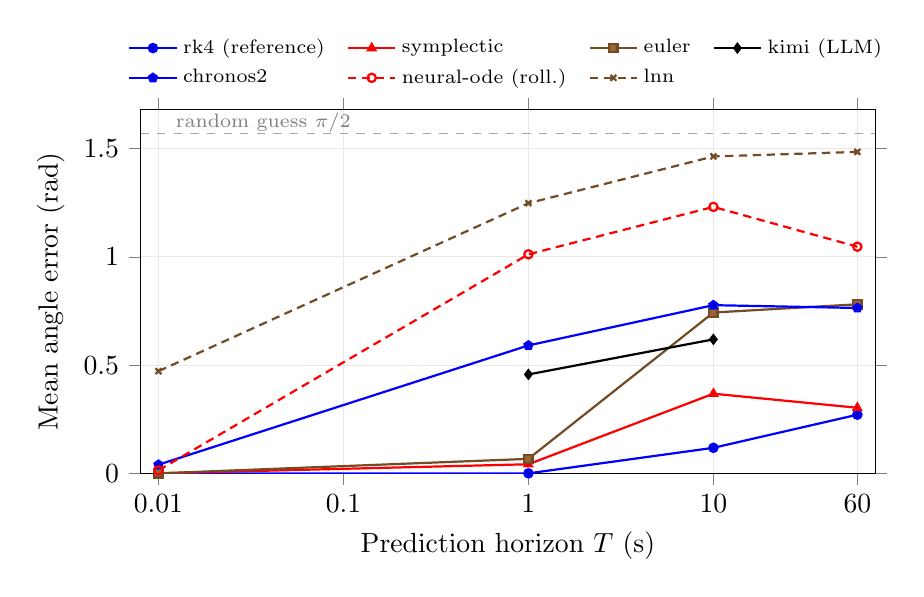
\begin{tikzpicture}
\begin{semilogxaxis}[
  width=0.9\linewidth, height=6.2cm,
  xlabel={Prediction horizon $T$ (s)}, ylabel={Mean angle error (rad)},
  xmin=0.008, xmax=75, ymin=0, ymax=1.68,
  xtick={0.01,0.1,1,10,60}, log ticks with fixed point,
  legend columns=4,
  legend style={at={(0.5,1.03)}, anchor=south, font=\scriptsize, draw=none, fill=none,
                cells={anchor=west}, /tikz/every even column/.append style={column sep=6pt}},
  grid=both, grid style={gray!18}, tick align=outside,
  every axis plot/.append style={thick, mark size=1.5pt},
]
\addplot+[mark=*]         coordinates {(0.01,0.000) (1,0.000) (10,0.118) (60,0.271)};
\addlegendentry{rk4 (reference)}
\addplot+[mark=triangle*] coordinates {(0.01,0.000) (1,0.042) (10,0.368) (60,0.303)};
\addlegendentry{symplectic}
\addplot+[mark=square*]   coordinates {(0.01,0.000) (1,0.067) (10,0.743) (60,0.781)};
\addlegendentry{euler}
\addplot+[mark=diamond*]  coordinates {(1,0.457) (10,0.619)};
\addlegendentry{kimi (LLM)}
\addplot+[mark=pentagon*] coordinates {(0.01,0.040) (1,0.591) (10,0.777) (60,0.764)};
\addlegendentry{chronos2}
\addplot+[mark=o]         coordinates {(0.01,0.014) (1,1.012) (10,1.231) (60,1.047)};
\addlegendentry{neural-ode (roll.)}
\addplot+[mark=x]         coordinates {(0.01,0.472) (1,1.248) (10,1.464) (60,1.485)};
\addlegendentry{lnn}
\draw[dashed, gray!70] (axis cs:0.008,1.5708) -- (axis cs:75,1.5708);
\node[anchor=west, gray, font=\scriptsize] at (axis cs:0.011,1.62) {random guess $\pi/2$};
\end{semilogxaxis}
\end{tikzpicture}
\caption{Error growth with prediction horizon (out-of-sample, reliability-adjusted; log time
axis). The numerical integrators stay near zero until ${\sim}10$\,s; every black-box family
saturates near the chaotic noise floor by $1$\,s. LLMs are evaluated at $\{1,10\}$\,s only.
Dashed line: random-guess baseline $\pi/2$.}
\label{fig:errorgrowth}
\end{figure}

\begin{table}[tbp]
\centering\small
\caption{Physical regimes. The \texttt{changed\_hidden} regime withholds the constants.}
\label{tab:regimes}
\begin{tabular}{lccccc}
\toprule
Regime & $g$ (m/s$^2$) & $L$ (m) & $m$ (kg) & damping & disclosed \\
\midrule
\texttt{normal} & 9.81 & 1.0 & 1.0 & 0.0 & --- \\
\texttt{changed\_disclosed} & 3.71 & 1.4/0.7/1.1 & 2.0/0.6/1.5 & 0.05 & yes \\
\texttt{changed\_hidden} & 1.62 & 0.8/1.2/0.9 & 0.5/1.8/1.0 & 0.10 & no \\
\bottomrule
\end{tabular}
\end{table}

\begin{table}[tbp]
\centering\small
\caption{Nested training-budget study. Reliability-adjusted pendulum error (rad), averaged
over three training initializations and two held-out seeds. Intervals come from hierarchical resampling over
initializations and held-out seeds. HNN is evaluated on the undamped normal regime only.}
\label{tab:budget}
\begin{tabular}{llrcc}
\toprule
Model & Scope & Total trajectories & Error & 95\% CI \\
\midrule
HNN & normal & 3 & 1.269 & [1.209, 1.349] \\
HNN & normal & 15 & 0.974 & [0.891, 1.062] \\
HNN & normal & 60 & 0.981 & [0.856, 1.113] \\
Neural ODE & all regimes & 9 & 1.090 & [1.011, 1.207] \\
Neural ODE & all regimes & 45 & 0.968 & [0.923, 1.028] \\
Neural ODE & all regimes & 180 & 0.861 & [0.829, 0.907] \\
\bottomrule
\end{tabular}
\end{table}

\begin{table}[tbp]
\centering\small
\caption{Training-objective study, out-of-sample mean angle error (rad) on the shared
held-out grid (horizons $\{1,10\}$\,s); architecture fixed, loss/window varied. Significance
from a powered paired study on the full four-horizon held-out set ($n{=}720$,
Wilcoxon$+$Holm).}\label{tab:objective}
\begin{tabular}{llcl}
\toprule
Model & Objective & Err & vs.\ prev.\ row \\
\midrule
\multirow{3}{*}{Neural ODE}
 & derivative MSE & 1.110 & --- \\
 & rollout (single-$k$) & 1.121 & n.s.\ ($p_{\mathrm{Holm}}{=}0.188$) \\
 & mixed-window & 1.036 & sig.\ ($p_{\mathrm{Holm}}{=}0.013$) \\
\midrule
\multirow{3}{*}{HNN}
 & derivative MSE & 1.138 & --- \\
 & rollout (single-$k$) & 0.972 & sig.\ ($p_{\mathrm{Holm}}{=}1.95{\times}10^{-4}$) \\
 & mixed-window & 1.066 & sig.\ higher ($p_{\mathrm{Holm}}{=}0.014$) \\
\bottomrule
\end{tabular}
\end{table}

\begin{table}[tbp]
\centering\small
\caption{Physical fidelity on the undamped (\texttt{normal}) regime: mean absolute energy
drift over a $10$\,s rollout, normalized by $E^{*}{=}g\sum_i m_i L_i$ (0 = perfect
conservation), and fraction of bounded rollouts. HNN drift is nearly unchanged when its rollout
uses a symplectic integrator.}\label{tab:energy}
\begin{tabular}{llcc}
\toprule
Model & Family & Energy drift & Stable \\
\midrule
rk4 & numerical & 0.000 & 100\% \\
symplectic & numerical & 0.066 & 100\% \\
euler & numerical & 0.494 & 100\% \\
neural-ode-rollout-mixed & learned & 0.779 & 100\% \\
hnn-rollout-mixed & learned & 0.865 & 100\% \\
neural-ode-rollout & learned & 0.872 & 100\% \\
hnn-rollout & learned & 2.065 & 100\% \\
lnn & learned & 4.038 & 27\% \\
hnn & learned & 4.270 & 100\% \\
neural-ode & learned & 4.346 & 100\% \\
\bottomrule
\end{tabular}
\end{table}

\begin{table}[tbp]
\centering\small
\caption{Out-of-sample mean angle error (rad) by horizon, reliability-adjusted, on the
shared held-out grid (selected models). The cross-family comparison uses horizons
$\{1,10\}$\,s.}\label{tab:horizon}
\begin{tabular}{lcc}
\toprule
Model & 1\,s & 10\,s \\
\midrule
rk4 (reference) & 0.000 & 0.118 \\
symplectic & 0.042 & 0.368 \\
euler & 0.067 & 0.743 \\
kimi-k2.6 & 0.457 & 0.619 \\
chronos2-multi & 0.591 & 0.777 \\
chronos2-uni & 0.622 & 0.773 \\
grok-4-1-fast-reasoning & 0.905 & 0.857 \\
deepseek-v4-pro & 0.996 & 0.909 \\
hnn-rollout & 0.855 & 1.088 \\
neural-ode-rollout-mixed & 0.951 & 1.120 \\
hnn-rollout-mixed & 0.982 & 1.150 \\
neural-ode & 0.892 & 1.328 \\
neural-ode-rollout & 1.012 & 1.231 \\
hnn & 1.052 & 1.224 \\
lnn & 1.248 & 1.464 \\
\bottomrule
\end{tabular}
\end{table}

\begin{table}[tbp]
\centering\small
\caption{Predictability horizon (s): longest horizon tracked contiguously below threshold
$\tau$, on the shared out-of-sample set (ladder $\{0.01,1,10,60\}$\,s). Higher is better;
``---'' means not even the first horizon stays below $\tau$.}\label{tab:predhorizon}
\begin{tabular}{lcccc}
\toprule
Model & $\tau{=}0.1$ & $0.25$ & $0.5$ & $1.0$ \\
\midrule
rk4 (reference) & 1.0 & 10 & 60 & 60 \\
symplectic & 1.0 & 1.0 & 60 & 60 \\
euler & 1.0 & 1.0 & 1.0 & 60 \\
neural-ode-rollout & 0.01 & 0.01 & 0.01 & 0.01 \\
neural-ode-rollout-mixed & 0.01 & 0.01 & 0.01 & 1.0 \\
chronos2-multi & 0.01 & 0.01 & 0.01 & 60 \\
chronos2-uni & 0.01 & 0.01 & 0.01 & 60 \\
hnn-rollout & 0.01 & 0.01 & 0.01 & 1.0 \\
neural-ode & 0.01 & 0.01 & 0.01 & 1.0 \\
hnn & 0.01 & 0.01 & 0.01 & 0.01 \\
lnn & --- & --- & 0.01 & 0.01 \\
\bottomrule
\end{tabular}
\end{table}

\section{Real-data check details}
\label{app:realdata}
The hardware dataset \citep{myers2020pendulum} is openly released via Mendeley Data
(CC~BY~4.0 listing; the deposit includes a GPLv3 license file) with video tracking of
both link angles at $500$\,Hz and per-frame uncertainty estimates (median $0.20^{\circ}$ upper
link, $0.43^{\circ}$ lower). We use the published simplified point-mass parameters
($L=[0.172,0.143]$\,m, $m=[0.311,0.111]$\,kg, $g=9.81$\,m/s$^2$). Angular velocities come from a
Savitzky--Golay filter (window $42$\,ms, cubic, analytic derivative). The recordings begin
with the pendulum positioned by hand, so the free drop is detected as the first time either
link exceeds $4$\,rad/s; evaluation states are drawn evenly from $0.2$ to $24$\,s after the
drop, $60$ per trial. The tracker zeroes its angle at the first frame, leaving a
gravity-referenced offset per link; every trial ends hanging at rest with tracked angles at
exact multiples of $360^{\circ}$ (within $0.08^{\circ}$), which fixes the offset at zero
independently of any model. A $20$\,ms physics-tracking check agrees, with error of
$0.005$--$0.007$\,rad against a $0.006$\,rad tracking floor. A grid search over
$\{0,5{\times}10^{-4},\dots,2{\times}10^{-2}\}$ selects damping $10^{-3}$ on Trial~1 at the $0.5$\,s
horizon. SINDy uses a degree-two polynomial plus first-order Fourier library on Trial~1 with
Savitzky--Golay derivatives; Chronos-2 receives a $5$\,s context resampled to $50$\,Hz and
forecasts at most $50$ steps. Failures are scored at $\pi/2$; Chronos-2's are input-infeasible cells (insufficient
context) rather than divergences, and the fixed-coverage rule scores both alike. The tracking
dataset has been public since 2020 and may appear in foundation-model corpora; contamination
would inflate Chronos-2's score, so its baseline-level result is, if anything, conservative. Paired
bootstrap differences over the $120$ states at $1.0$\,s: RK4 minus persistence $+0.018$
($95\%$ CI $[-0.121,+0.155]$); damped minus undamped RK4 $-0.103$ ($[-0.202,-0.003]$), so
the damping gain at the longest horizon is significant while the RK4--persistence gap is
not. States sampled along a trajectory are temporally dependent, so we repeat both with a
moving-block bootstrap within each trial (blocks of $10$ consecutive states, ${\sim}4$\,s):
the conclusions are unchanged (damped minus RK4 $[-0.179,-0.019]$; RK4 minus persistence
$[-0.131,+0.064]$), and remain so for block lengths from $2$ to $12$\,s.

\begin{table}[tbp]
\centering\small
\caption{Real-data check: mean wrapped angle error (rad) over both links on Trials 2--3
($120$ held-out states), failures at $\pi/2$. The physics rows use the published constants;
``damped'' adds the Trial-1-fitted viscous coefficient. Tracking noise floor
${\sim}0.006$\,rad.}
\label{tab:realdata}
\begin{tabular}{lcccc}
\toprule
Model & $0.1$\,s & $0.5$\,s & $1.0$\,s & Answered \\
\midrule
physics-rk4 & 0.084 & 0.820 & 1.248 & 100\% \\
physics-rk4-damped & 0.086 & 0.892 & 1.145 & 100\% \\
nearest-neighbor (cross-trial) & 0.371 & 0.849 & 1.117 & 100\% \\
chronos2 & 0.611 & 1.160 & 1.223 & 89\% \\
constant-velocity & 0.345 & 1.402 & 1.576 & 100\% \\
sindy-real & 0.490 & 1.501 & 1.535 & 99\% \\
persistence & 0.934 & 1.654 & 1.230 & 100\% \\
\bottomrule
\end{tabular}
\end{table}

\end{document}
